\documentclass[a4paper, 14pt]{report}

\usepackage{cmap}
\usepackage[T2A]{fontenc}
\usepackage[utf8]{inputenc}
\usepackage[english,russian]{babel}
\usepackage[left=30mm, top=20mm, right=20mm, bottom=20mm, nohead, nofoot]{geometry}
\usepackage{indentfirst}

\usepackage{amsmath}
\usepackage{MnSymbol}
\usepackage{wasysym}
\usepackage{float}

\usepackage{pgfplots}

\usepackage{tikz}
\usetikzlibrary{graphs}

\usepackage{graphicx}
\graphicspath{{img/}}
\DeclareGraphicsExtensions{.pdf}

\usepackage[most]{tcolorbox}
\newtcolorbox{lbox}[2][] {
    enhanced,
    %fonttitle=\ttfamily,
    %fontupper=\ttfamily,
    sharp corners,
    colback=white,
    colbacktitle=white,
    coltitle=black,
    boxed title style={colframe=white},
    attach boxed title to top center={yshift=-3mm},
    title=#2,#1
}

\author{Гаврилова Юлия Михайловна}
\title{Базы данных}
\date{2019}

\begin{document}
\maketitle

\tableofcontents
\clearpage

\chapter{Введение}

\begin{center}
\begin{tabular}{|c|c|}
    \hline
    \multicolumn{2}{|c|}{Способы организации} \\
    \hline
    \textbf{OLAP} (online analytic processor) & \textbf{OLTP} (jnline transaction processor) \\
    \hline
    Время отклика & Быстрая вставка \\
    \hline
    3NF & 1NF \\
    \hline
    Нормальная форма & Для сбора статистики \\
    \hline
\end{tabular}
\end{center}

\begin{tikzpicture}
    \graph[nodes={align=center,rectangle,draw=black}, grow down sep, branch right sep]
    {
        SQL -> "Reluationnaya model" ->
        {
            "Teoria mnozestv",
            "Teoria predikatov"
        }
    };
\end{tikzpicture}

\hfill

\begin{tikzpicture}
    \graph[nodes={align=center,rectangle,draw=black}, grow down sep, branch right sep]
    {
        SYBD -> BD
    };
\end{tikzpicture}

\section{Реляционная модель}

\begin{enumerate}
    \item Стректурная часть: как построена модель
    \item Целостная часть: какие ограничения, как должны быть организованы данные
    \item Манипуляционная: обработка данных
\end{enumerate}

\subsection{Структурная часть}

\begin{itemize}
    \item Тип int, char
    \item домен - надстройка над типом, набор ограничений/правил (положительные четные для int), можно объявить над типом или над доменом
    \item атрибут - упорядоченная пара (<имя, тип или домен>)
    \item заголовок (схема) отношения - множество всех пар атрибутов \{<имя атрибута$_1$, значение$_1$>,$\dots$, <имя атрибута$_N$, значение$_N$>\}

        \{<$a_1$, int>,<$a_2$, float>,<$a_3$, char>,<$a_4$, varchar>\}
    \item кортеж над схемой

        \{<$a_1$, 1>,<$a_2$, 1.4>,<$a_3$, 'a'>,<$a_4$, 'aaa'>\}
    \item отношение

        \begin{tabular}{|c|c|c|c|}
            \hline
            $a_1$ & $a_2$ & $a_3$ & $a_4$ \\
            \hline
            1 & 1.4 & 'a' & 'aaa' \\
            \hline
        \end{tabular}
\end{itemize}


\paragraph{ER-модель}

\begin{itemize}
    \item отношение/сущность

        \begin{tikzpicture}
            \graph[nodes={align=center,rectangle,draw=black}, grow down sep, branch right sep]
            {
                students -> "second name",
                students -> "group",
                students -> tails,
                students -> number
            };
        \end{tikzpicture}
\end{itemize}

Здесь студент сущность сильная. Если студент зависит, то студент - слабая сущность

\begin{itemize}
    \item связь 1 - 1 (Студент $\to$ зачетка)
    \item связь 1 ко многим (Студенты $\to$ группа)
    \item многие ко многим (Студенты $\to$ курс)
\end{itemize}

\begin{lbox}{\textbf{Лабораторная работа 1}}
    \begin{itemize}
        \item Подобрать предметную область на весь семестр
        \item ER модель (не менее 3ч самостоятельных сущностей)
        \item Создать свою БД (не менее 1000 записей на таблицу)
    \end{itemize}
    \textbf{Защита:}
    \begin{itemize}
        \item Добавить связь/атрибут
        \item Создать ссылку
    \end{itemize}
\end{lbox}

\subsection{Целостная часть}

\begin{itemize}
    \item целостность сущностей/отношений
    \item целостность ссылок

        \begin{tabular}{|c|c|c|}
            \hline
            id & ФИО & Age \\
            \hline
            1 & Иванов & 10 \\
            \hline
            2 & Петров & 15 \\
            \hline
            3 & Иванов & 45 \\
            \hline
        \end{tabular}
\end{itemize}

Потенциальный ключ:

\begin{itemize}
    \item однозначная идентификация записи
    \item никаких подмножеств не должно быть под ключом
\end{itemize}

\begin{center}
    \begin{tabular}{|c|c|c|}
        \hline
        id & ФИО & id группы \\
        \hline
        1 & Петров & 1 \\
        \hline
        & & \\
        \hline
    \end{tabular}

    $\downarrow$ Внешняя ссылка

    \begin{tabular}{|c|c|}
        \hline
        id & Название \\
        \hline
        1 & ИУ7-53 \\
        \hline
        & \\
        \hline
    \end{tabular}
\end{center}

Ссылочная целостность - нельзя ссылаться на несуществующий объект

\subsection{Манипуляционная часть}

\begin{itemize}
    \item Реляционная алгебра
    \item Реляционные исчисления
\end{itemize}

\section{Реляционная алгебра}

\begin{tabular}{|c|c|}
    \hline
    id & name \\
    \hline
    1 & a \\
    \hline
    2 & b \\
    \hline
\end{tabular}

\hfill

\begin{tabular}{|c|c|}
    \hline
    id & name \\
    \hline
    2 & b \\
    \hline
    3 & c \\
    \hline
\end{tabular}

\begin{enumerate}
    \item Традиционные - работа с множеством

        \begin{itemize}
            \item Объединение (UNION)

                \begin{tabular}{|c|c|}
                    \hline
                    id & name \\
                    \hline
                    1 & a \\
                    \hline
                    2 & b \\
                    \hline
                    3 & c \\
                    \hline
                \end{tabular}

            \item Пересечение (INTERSECT)

                \begin{tabular}{|c|c|}
                    \hline
                    id & name \\
                    \hline
                    2 & b \\
                    \hline
                \end{tabular}

            \item Вычитание (MINUS)

                \begin{tabular}{|c|c|}
                    \hline
                    id & name \\
                    \hline
                    1 & a \\
                    \hline
                \end{tabular}

                \begin{tabular}{|c|c|}
                    \hline
                    id & name \\
                    \hline
                    3 & c \\
                    \hline
                \end{tabular}

            \item Декартово произведение (TIMES) - все возможные комбинации атрибутов
        \end{itemize}

    \item Специальные

        \begin{itemize}
            \item Соединение (JOIN)

                \begin{tabular}{|c|c|c|}
                    \hline
                    id & name1 & name2\\
                    \hline
                    2 & b & b \\
                    \hline
                \end{tabular}

            \item Ограничение (WHERE)
            \item Проекция (PROJECT)
            \item Деление (DIVIDE BY)
        \end{itemize}
\end{enumerate}

Реляционное выражение = унарное выражение (бинарное выражение)

\paragraph{Унарные выражения}

\begin{itemize}
    \item Проекция

        терм | терм[список атрибутов]

    \item Ограничение

        терм WHERE логическое\_выражение

    \item Переименование

        терм RENAME old\_name TO new\_name

\end{itemize}

терм - имя\_отношения | (реляционное\_выражение)

\paragraph{Бинарные выражения}

\begin{itemize}
    \item Объединение
    \item Пересечение
    \item Вычитание
    \item Декартово произведение
    \item Соединение
\end{itemize}

бинарные операции = проекция бинарная\_операция реляцонное\_выажение

S JOIN P[P..,S..]

\begin{tabular}{|c|}
    \hline
    Поставщик \\
    \hline
    S \\
    \hline
\end{tabular}

$ \downarrow $ Многие ко многим SP

\begin{tabular}{|c|}
    \hline
    Детали \\
    \hline
    P \\
    \hline
\end{tabular}

\hfill

$S(Sno : integer, Sname : string, Status : integer, City : string)$

$P(Pno : integer, Pname : string, Color : string, Weight : real, City : string)$

$SP(Sno : integer, Pno : integer, Quantity : integer)$

\paragraph{S}

\hfill

\begin{tabular}{|c|c|c|c|}
    \hline
    Sno & Sname & Status & City \\
    \hline
    1 & Алмаз & 20 & Смоленск \\
    2 & Дельта & 10 & Владимир \\
    3 & Орион & 30 & Смоленск \\
    \hline
\end{tabular}

\paragraph{P}

\hfill

\begin{tabular}{|c|c|c|c|c|}
    \hline
    Pno & Pname & Color & Weight & City \\
    \hline
    1 & Гайка & К & 12.0 & Смоленск \\
    2 & Болт & С & 17.1 & Рязань \\
    3 & Винт & З & 15.47 & Владимир \\
    4 & Винт & К & 18 & Москва \\
    5 & Шайба & З & 25 & Смоленск \\
    \hline
\end{tabular}

\paragraph{SP}

\hfill

\begin{tabular}{|c|c|c|}
    \hline
    Sno & Pno & Quantity \\
    \hline
    1 & 1 & 25 \\
    1 & 2 & 14 \\
    2 & 4 & 2 \\
    \hline
\end{tabular}

\begin{enumerate}
    \item Имена всех поставщиков детали под номером 2

        $$
        \underbrace{((\underbrace{\text{SP join S})}_\text{рел. выр.} \text{where} \underbrace{\text{Pno = 2}}_{\text{лог. выр.}})}_\text{реляционное выражение}[\text{Sname}]
        $$

        select Sname

        from SP inner join S on SP.Sno = S.Sno

        where SP.Pno = 2

    \item Вывести все имена поставщиков, которые поставляюк как минимум одну красную деталь

        $$
        (((\text{P where } \text{Color = 'К'}) \text{join SP}) \text{join S})[\text{Sname}]
        $$

    \item Получить имена поставщиков, которые поставляют все детали

        $A(X_1, \dots, X_n, Y_1, \dots, Y_n)$

        $B(Y_1, \dots, Y_n)$

        $A \text{ divide by } B = (X_1, \dots, X_n)$

        \begin{tabular}{|c|c|}
            \hline
            Sno & Pno \\
            \hline
            1 & 1 \\
            1 & 2 \\
            1 & 3 \\
            2 & 2 \\
            2 & 3 \\
            3 & 1 \\
            \hline
        \end{tabular}

        $P[Pno]$

        $SP \text{ divide by } P[Pno]$

        $((SP \text{ divide by } P[Pno]) \text{ join } S)[Sname]$

    \item Все поставщики, которые поставляют только красные детали

        $(Sp \text{divide by }(P \text{ where } \text{Color = 'К'})[Pno])[Sname]$

    \item Переименовать города из первой таблицы во вторые

        $(S \text{ rename } Sno \text{ to } firstName)[firstName, City] \text{ join }$

        $(S \text{ rename } Sno \text{ to } secondName)[secondName, City]) \text{ where } secondName > firstName \text{ join } S$

        \begin{tabular}{|c|c|}
            \hline
            firstName & C \\
            \hline
            1 & С \\
            2 & В \\
            3 & С \\
            \hline
        \end{tabular}

        \begin{tabular}{|c|c|}
            \hline
            secondName & C \\
            \hline
            1 & С \\
            2 & В \\
            3 & С \\
            \hline
        \end{tabular}

        \begin{tabular}{|c|c|c|}
            \hline
            firstName & secondName & C \\
            \hline
            1 & 1 & С \\
            1 & 3 & С \\
            2 & 2 & В \\
            3 & 1 & С \\
            3 & 3 & С \\
            \hline
        \end{tabular}

    \item Поставщики, которые не поставляют деталь номер 2

        $((S[Sno] \text{ minus } (SP \text{ where } Pno=2)[Sno]) \text{ join } S)[Sname]$

\end{enumerate}

\subsection{GROUP}

SP group (Pno, Qty) as PQ - группирует

\begin{tabular}{|c|c|c|}
    \hline
    Sno & Pno & Qty \\
    \hline
    1 & 1 & 10 \\
    \hline
    1 & 2 & 15 \\
    \hline
    2 & 1 & 5 \\
    \hline
\end{tabular}

$\downarrow$

\begin{tabular}{|c|c|}
    \hline
    Sno & PQ \\
    \hline
    1 & 1-10 2-15 \\
    \hline
    2 & 1-5 \\
    \hline
\end{tabular}

\subsection{Summarize}

summarize SP per SP \{Pno\} add sum(Qty) as sQty

\begin{tabular}{|c|c|}
    \hline
    Pno & sQty \\
    \hline
    1 & 15 \\
    \hline
    1 & 16 \\
    \hline
\end{tabular}

extend S add 'Поставщик' as Sname2

extend SP add Qty*100 as Qty2

\subsection{UNGROUP}

\section{Реляционное сравнение}

S(Sno) = SP(Sno)

is\_epmty(реляционное выражение)

t in R $\Leftrightarrow$ RELATION\{t\} $\le$ R

t - Кортеж

R - отношение

\begin{center}
    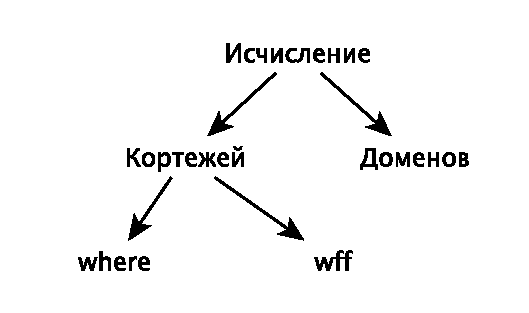
\includegraphics{db1}
\end{center}

объявление = range of переменная is список

область = отношение | реляционное выражение

реляционное выражение = (список целевых элементов) [where(wff)]

целевой элемент = переменная | переменная атрибут [as имя]

wff = условие | not условие | условие and (or) wff | if условие then(wff)

\paragraph{Примеры}

\hfill

range of SX is S

range of SPX is SP

range of SY is (SX) where SX.City = 'Смоленск', (SX) where exists SPX(SPX.Sno=SX.Sno and SPX.Pno=1)

Задачи как в реляционной алгебре

\begin{enumerate}
    \item range of SX is S (SPX.Sno) where SPX.Pno = 2 (SX.Sname) where exists SPX(SPX.Sno = SX.Sno and SPX.Pno = 2)
    \item range of SX os P (SX.Sname) where exists SPX(SPX.Sno = SX.Sno and exists PX(SPX.Pno = PS.Pno and PX.Color = 'К'))

        (SX.Sname) where exists SPX(where exists PX(SPX.Sno = SX.Sno and SPX.Pno = SX.Pno and PX.Color = 'к'))

        range of PX is (Pno) where P.Color = 'К'

    \item (SX.Sname) where forall PX(exists SPX(SPX.Pno = SX.Pno and SPX.Sno = SX.Sno))

    \item <$S_1$, $S_2$>

        range of SY is S (SX.Sname as FirstName, SY.Sname as SecondName) SX.City = SY.City and SX.Sno > SY.Sno

    \item (SX.Sname) where not exists SPX(SPX.Sno = SX.Sno and SPX.Pno = 2)
\end{enumerate}

\subsection{Агрегатные сравнения}

(sum(SPX.Qty) as Total)

агрегатная функция((атрибуты) where f[атрибуты])

\section{Исчисление доменов}

R(pair, pair...) - условие принадлежности в общем виде

R - имя отношения, pair = A:v, где A - атрибут отношения R, v - или переменная
домена, или литерал

SP(Sno : 1, Pno:1) - истина если есть кортеж с Sno = 1 и Pno = 1

SP(Sno:SX, Pno:PX) - только если в отношении SP есть кортеж

\begin{enumerate}
    \item (SX) - множество всех номеров поставщиков
    \item (SX) where S(Sno : SX) - множество всех номеров поставщиков в отношении S
    \item (SX) where S(Sno : SX, City : 'Смоленск') - подмножество номеров поставщиков из города Смоленска
    \item (SX,CityX) where S(Sno : SX, City : CityX) and SP(Sno : SX, Pno : 2) - запрос на получение номера поставщиков поставляющих деталь под номером 2
    \item (SX, PX) where S(Sno : Sx, City : CityX) and P(Pno : PX, City : CityY) and CityX <> CityY - получение пар номер поставщика и детали где поставщики и детали находятся не в одном городе
\end{enumerate}

\begin{enumerate}
    \item Получить номера поставщиков из Смоленска у которых статус больше 20

        SX where exists StatusX (StatusX > 20 and S(Sno : SX, Status : StatusX, City : 'Смоленск'))
    \item Получить все пары поставщиков, что два поставщика размещаются в одном городе

        (SX as FirstSno, SY as SecondSnno) where exists CityZ(S(Sno : SX, City : CityZ) and S(Sno : SY, City : CityZ) and SX < SY)

    \item Получить имена поставщиков которые поставляют как минимум одну красную деталь

        NameX where exists SX exists PX (S(Sno : SY, Sname : NameX) and SP(Sno : SX, Pno : PX) and P(Pno : PX, Color = 'Красный'))

    \item Получить имена поставщиков которые поставляют хотя бы одну деталь поставляемую поставщиком под номером 2

        NameX where exists SX exists PX (S(Sno : SX, Sname : NameX) and SP(Sno : SX, Pno : PX) and SP(Sno : 2, Pno : PX))

    \item Получить имена поставщиков которые поставляют все типы деталей

        NameX where exists SX(S(Sno : SXm Sname : NameX) and forall PX(if P(Pno : PX) then (Sno : SX, Pno : PX)))

    \item Получить имена поставщиков которые не поставляют деталь с номером 2

        NameX where exists SX(S(Sno : SX, Sname : NameX) and not SP(Sno : SX, Pno : 2))

    \item Получить номера поставщиков которые поставляют как минимум все типы деталей поставляемыми поставщиком с номером 2

        SX where forall PX(if SP(Sno : 2, Pno : PX) then SP(Sno : SX, Pno : PX))

    \item Получить номера деталей которые не весят больше 16 фунтов или поставляются с поставщиком под номером 2, или и то и другое

        PX where exists WeightX(P(Pno : PX, WeightX) and WeightX > 16) or SP(Sno : 2, Pno : PX))
\end{enumerate}

Поставщики (S)

\begin{tabular}{|c|c|c|c|}
    \hline
    Sno & Sname & Status & City \\
    \hline
    1 & Алмаз & 20 & Смоленск\\
    \hline
    2 & Циклон & 10 & Владивосток \\
    \hline
    \vdots & & & \\
\end{tabular}

Детали (P)

\begin{tabular}{|c|c|c|c|c|}
    \hline
    Pno & Pname & Color & Weight & City \\
    \hline
    1 & Гайка & Красный & 12 & Смоленск\\
    \hline
    2 & Болт & Зеленый & 17 & Владимир\\
    \hline
    $\vdots$ & & & & \\
\end{tabular}

Проекты (J)

\begin{tabular}{|c|c|c|}
    \hline
    Jno & Jname & City \\
    \hline
    1 & Ангара & Владимир \\
    \hline
    2 & Алтай & Рязань \\
    \hline
    $\vdots$ & & \\
\end{tabular}

Поставки (SPJ)

\begin{tabular}{|c|c|c|c|}
    \hline
    Sno & Pno & Jno & Qty \\
    \hline
    1 & 1 & 1 & 200 \\
    \hline
    1 & 1 & 4 & 700 \\
    \hline
    $\vdots$ & & & \\
\end{tabular}

\begin{enumerate}
    \item (SX,Name, SX.City) where exists JX forall PX exists PSJX (JX.City = 'Ярославль' and JX.Jno = SPJX.Jno and PX.Pno = SPJX.Pno and SX.Sno = SPJX and SPJX.Qty >= 50)

SX : все кортежи отношения S (5 шт)

PX : все кортежи отношения P (6 шт)

JX : все кортежи отношения J, в которых City = 'Ярославль' (2шт)

SPJX : все кортежи отношения SPJ, d которых Qty >= 50 (24 шт)

    \item JX.JN = SPJX.Jno and PX.Pno = SPJX.Ono and SX.Xno = SPJX.Sno

    \item exists RX, forall RX

    \item exists JX forall PX exists SPJX

\end{enumerate}

\begin{enumerate}
    \item exists SPJX исключая SPJ (SPJ.Sno, SPJ.Pno, SPJ.Jno и SPJ.Qty)

        \begin{tabular}{|c|c|c|c|c|c|c|c|c|c|c|c|}
            \hline
            Sno & Sname & City & Pno & Pname & Color & weight & City & Jno & Jname & City \\
            \hline
                & & & & & & & & & & \\
        \end{tabular}

    \item forall PX Делим на P

        \begin{tabular}{|c|c|c|c|c|c|c|}
            \hline
            Sno & Sname & Status & City & Jno & Jname & City \\
            \hline
                & & & & & & \\
        \end{tabular}

    \item exists JX исключаем J(J.Jno, J.Jname, J.City)

        \begin{tabular}{|c|c|c|c|}
            \hline
            Sno & Sname & Status & City \\
            \hline
                & & & \\
        \end{tabular}

    \item[5.] SX.Sname, SX.City

        \begin{tabular}{|c|c|}
            \hline
            Sname & City \\
            \hline
                  & \\
        \end{tabular}
\end{enumerate}

\chapter{Теория проектирования реляционных баз данных}

Есть две проблемы: как повсить эффективность и как представить реальные объекты.

Классический подход это выделение решений и их реализация. Нормальные формы. каждая НФ - набор ограничений. Каждая следующая НФ лучше предыдущей.

Следующие нормальные формы:

\begin{enumerate}
    \item 1 NF
    \item 2 NF
    \item 3 NF
    \item 4 NF
    \item PSNF - форма проекций соединения
\end{enumerate}

\paragraph{Свойства НФ}

\begin{enumerate}
    \item Каждая следующая НФ лучше предыдущей
    \item При переходе к следующей НФ, свойства предыдущей сохраняются
\end{enumerate}

\paragraph{РК}

\begin{enumerate}
    \item ER модель
    \item Рел. алг., МК, SQL
    \item Функц. зависимости
\end{enumerate}

\paragraph{Доп задача на 3 балла}

Есть столбец с id с числами. Нужно вычислить произведение SQL

\section{Функциональная зависимость}

$x \to y$

\begin{tabular}{|c|c|c|}
    \hline
    Pno & Pname & Color \\
    \hline
        &       &       \\
\end{tabular}


Pno $\to$ Pname

Pno $\to$ Color

\subsection{Правила для функциональных зависимостей}

\begin{enumerate}
    \item $(B \subset A) \Rightarrow A \to B$
    \item $A \to B \Rightarrow AC \to BC$
    \item $A \to B \text{ и } B \to C \Rightarrow A \to C$
    \item $A \to A$
    \item $A \to BC \Rightarrow A \to B \text{ и } A \to C$
    \item $A \to B \text{ и } A \to C \Rightarrow A \to BC$
    \item $A \to B \text{ и } C \to B \Rightarrow AC \to BD$
    \item $A \to B \text{ и } C \to D \Rightarrow A(C - B) \to BD$
\end{enumerate}

R -- переменная отношения

R(A,B,C,D,E,F)

S = $\{ A \to BC, B \to E, CD \to EF \}$ -- набор функциональных зависимостей

$AD \to F ?$

$\{AD\}^+$ -- замыкание атрибутов

\begin{tabular}{|c|c|c|}
    \hline
    & Jold = Jnew = $\{ A,D \}$ & Jold=Jnew = $\{ A,B,C,D,E,F \}$\\
    \hline
    $A \to BC$ & $A,B,C,D$ & - -//- - \\
    \hline
    $B \to E$ & $A,B,C,D,E$ & - -//- - \\
    \hline
    $CD \to EF$ & $A,B,C,D,E,F$ = Jnew & - -//- - \\
    \hline
\end{tabular}

\begin{enumerate}
    \item $A \to BC \Rightarrow A \to B \text{ и } A \to C$
    \item $AD \to CD$
    \item $AD \to CD \text{ и } CD \to EF \Rightarrow AD \to EF$
    \item $AD \to EF \Rightarrow AD \to E \text{ и } \underline{AD \to F }$
\end{enumerate}

\paragraph{}

$$
F =
\left\{
    \begin{matrix}
        A \to C,  \\
        AC \to D, \\
        E \to AD, \\
        E \to H   \\
    \end{matrix}
\right\}
$$

$$
G =
\left\{
    \begin{matrix}
        A \to CD, \\
        E \to AH  \\
    \end{matrix}
\right\}
$$

$F?G$

\begin{enumerate}
    \item $\overbrace{\{A\}^+}^{\text{Детерминант } F} = \overbrace{\{A,C,D\}}^{\text{По } F} = A \to CD (\text{из } G)$

        $\{AC\}^{-1} = \{A,C,D\} = A \to CD$

        $\{E\}^+ = \{E,A,D,H,C\} = E \to AH (\text{из } G)$

    \item $\{A\}^+ = \{A,C,D\} = AC \to D$

        $\{E\}^+ = \{A,C,D,E,H\} = E \to AD \text{ и } E \to H$
\end{enumerate}

$F = G$

\paragraph{Поиск минимального покрытия}

$R(A,B,C,D)$

$$
S =
\left\{
    \begin{matrix}
        A \to BC, \\
        B \to C,  \\
        A \to B,  \\
        AB \to C, \\
        AC \to D  \\
    \end{matrix}
\right\}
$$

\begin{itemize}
    \item Справа 1 элемент
    \item Нет транзитивных, тривиальных, выводимых зависимостей
    \item Слева все детерминанты приведены к минимальному виду
\end{itemize}

$$
\begin{matrix}
    A  \to B   &                        \\
    A  \to C   &  \text{транзитивность} \\
    B  \to C   &                        \\
    A  \to B   &  \text{дубль}          \\
    AB \to C   &  \text{выводима}        \\
    AC \to D   &                         \\
\end{matrix}
$$

$$
A \to B, B \to C, A \to D
$$

\section{Нормализация}

\begin{itemize}
    \item Избавление от аномалий

        \begin{itemize}
            \item обновление
            \item удаление
            \item вставка
        \end{itemize}

    \item Минимизировать объем данных
\end{itemize}

\subsection{Первая нормальная форма}

\begin{itemize}
    \item Атрибуты атамарны

        \begin{tabular}{|c|c|c|}
            \hline
            ФИО & Город & Телефон \\
            \hline
            Иванов & Москва & 8-916-... \\
                   &        & 8-925-... \\
            \hline
        \end{tabular}

        \begin{tabular}{|c|c|c|}
            \hline
            ФИО & Город & Телефон \\
            \hline
            Иванов & Москва & 8-916-... \\
            \hline
            Иванов & Москва & 8-925-... \\
            \hline
        \end{tabular}

        
\includegraphics{db2}

        \begin{tabular}{|c|c|}
            \hline
            ФИО & Город \\
            \hline
            Иванов & Москва \\
            \hline
        \end{tabular}

        \begin{tabular}{|c|c|}
            \hline
            id & Номер \\
            \hline
            1 & 8-916-... \\
            \hline
            1 & 8-925-... \\
            \hline
        \end{tabular}

\end{itemize}

\subsection{Вторая нормальная форма}

\begin{itemize}
    \item 1NF
    \item Каждый неключевой атрибут зависит от ключа

        \begin{tabular}{|c|c|c|c|c|}
            \hline
            Код поставки & Город & Страна города & Код товара & Кол-во \\
            \hline
            1 & М & 20 & 1 & 300 \\
            1 & М & 20 & 2 & 400 \\
            1 & М & 20 & 3 & 100 \\
            2 & Я & 10 & 4 & 200 \\
            3 & С & 30 & 5 & 300 \\
            3 & С & 30 & 6 & 400 \\
            4 & П & 15 & 7 & 100 \\
            \hline
        \end{tabular}

        \{КП, КТ\} $\to$ \{Кол-во\}

        КП $\to$ Город

        КП $\to$ Статус

        Город $\to$ Статус

        \begin{table}[H]
            \centering
            \begin{tabular}{|c|c|c|}
                \hline
                КП & КТ & Кол-во \\
                \hline
                1 & & \\
                1 & & \\
                2 & & \\
                3 & & \\
                3 & & \\
                4 & & \\
                \hline
            \end{tabular}
        \end{table}
        \end{itemize}

\subsection{Третья нормальная форма}

\begin{itemize}
    \item 2НФ
    \item Не должно быть транзитивных зависимостей
\end{itemize}

\begin{table}[H]
    \centering
    \begin{tabular}{|c|c|c|}
        \hline
        Сотрудник & Отдел & Номер телефона \\
        \hline
        Иванов & ИТ & 900 \\
        Петров & ИТ & 900 \\
        Сидоров & Бехгалтерия & 901 \\
        \hline
    \end{tabular}
\end{table}

\{Сотрудник\} $\to$ \{Отдел\}

\{Сотрудник\} $\to$ \{Телефон\}

\{Отдел\} $\to$ \{Телефон\}

\subsection{НФ Бойса-Кодда}

Каждая функциональная зависимость имеет в качестве своего детерминанта некий потенциальный ключ.

\begin{table}[H]
    \centering
    \begin{tabular}{|c|c|c|c|}
        \hline
        № Корта & Начало & Конец & Тариф \\
        \hline
        1 & 9:00  & 10:30 & + \\
        1 & 10:00 & 11:30 & + \\
        1 & 11:00 & 12:30 & - \\
        2 & 10:00 & 11:30 & + \\
        2 & 11:00 & 12:30 & + \\
        2 & 15:00 & 16:30 & - \\
        \hline
    \end{tabular}
\end{table}

Потенциальные ключи:

\begin{itemize}
    \item \{№, начало\}
    \item \{№, конец\}
    \item \{Тариф, начало\}
    \item \{Тариф, конец\}
\end{itemize}

$\Rightarrow$ \{№,\} $\to$ \{тариф\}

\begin{table}[H]
    \centering
    \begin{tabular}{|c|c|c|}
        \hline
        № Корта & Начало & Конец \\
        \hline
        & & \\
    \end{tabular}

    \begin{tabular}{|c|c|}
        \hline
        № Корта & Тариф \\
        \hline
                & \\
    \end{tabular}
\end{table}

\subsection{Четвертая нормальная форма}

Отношение находится в четвертой нормальной форме тогда и только тогда, когда все
нетривиальные многозадачные зависимости представляют собой функциональные зависимости
от ее ключей.

\begin{table}[H]
    \centering
    \begin{tabular}{|c|c|c|}
        \hline
        Курс & Книга & Лектор \\
        \hline
        Инф & К1 & Иванов \\
        Инф & К2 & Петров \\
        Инф & К3 & Сидоров \\
        \hline
    \end{tabular}
\end{table}

\subsection{Пятая нормальная форма}

Отношение находится в 5 НФ (проекционно-соед.) тогда и только тогда,
когда каждая нетривиальная зависимость определяется потенциальным
ключом этой зависимости.

\section{Методы физического хранения данных на диске}

Данные можно хранить построчно, тогда важна именно строка

\subsection{MPP (GreenPlum)}

\section{Транзации}

Это набор действий, которые выполняются как единое целое.

ACID

\begin{enumerate}
    \item А - атомарность
    \item C - консистентность
    \item I - изолированность
    \item D - долговечность
\end{enumerate}

\end{document}
